\chapter{Stand der Forschung / Stand der Technik}

In diesem Kapitel soll der Bezug der Arbeit zum aktuellen Stand der Forschung, bzw. zum Stand der Technik, je nach Ausrichtung und Schwerpunkt der Arbeit, verdeutlicht werden. Dazu werden entsprechende Vorarbeiten oder alternative Ansätze vorgestellt und diskutiert. Ziel ist es, den Ansatzpunkt der Arbeit genauer zu bestimmen und etwaige Entscheidungen im späteren Verlauf des Textes zu fundieren.

Dieses Kapitel kann je nach Thema der Arbeit {\emph Stand der Forschung} oder
{\emph Stand der Technik} heißen. In jedem Kapitel ist es wichtig, wie hier
geschehen zu Beginn kurz zu erläutern, um was es in diesem Kapitel geht.

Typischer Umfang des Stands der Forschung: 2-4 Seiten BA, 10-15 Seiten MA.

\section{Virtual Reality}

Der Begriff "Virtual Reality (VR)" wird in der Literatur nicht einheitlich definiert \citep{wohlgenannt_virtual_2020}. Es existieren verschiedene Definitionen, die unterschiedliche Aspekte der Technologie betonen. So wird VR beispielsweise von Berg und Vance als eine Sammlung von Technologien beschrieben, die es Menschen ermöglichen, immersiv eine Welt jenseits der Realität zu erleben. 
Nach Bowman und McMahan (2007) simuliert VR eine virtuelle Umgebung, die den Nutzenden das Gefühl vermittelt, "dort zu sein". Jerald (2016) definiert VR hingegen als eine computergenerierte digitale Umgebung, die erlebt und interagiert werden kann, als ob diese Umgebung real wäre. In ihrer Definition von VR führen \citet{wohlgenannt_virtual_2020} die verschiedenen Ansätze zur Beschreibung von VR zusammen und präzisieren, dass VR immersive Technologien nutzt, um interaktive virtuelle Umgebungen oder virtuelle Welten zu simulieren, in die sich die Nutzenden subjektiv einbringen und in denen sie sich physisch anwesend fühlen.

Des Weiteren identifizieren \citet{walsh_virtual_2002} Immersion, Interaktivität und Präsenz als drei zentrale Konzepte von VR. Der Begriff der Präsenz wird definiert als "die subjektive Erfahrung, sich an einem Ort oder in einer Umgebung zu befinden, auch wenn man physisch an einem anderen Ort ist" \citep{witmer_measuring_1998}. In einer virtuellen Umgebung entsteht das Gefühl von Präsenz insbesondere durch die Verlagerung der Aufmerksamkeit von der physischen auf die virtuelle Umgebung, wobei jedoch keine vollständige Ablösung von der physischen Realität notwendig ist \citep{witmer_measuring_1998}. 

Im Gegensatz zur Präsenz ist der Begriff der Immersion weniger eindeutig definiert. \citet{witmer_measuring_1998} beispielsweise definieren Immersion als einen psychologischen Zustand, in dem eine Person sich als umhüllt und in eine Umgebung eingebunden empfindet, die kontinuierliche Reize und Erfahrungen liefert. \citet{sanchez-vives_presence_2005} hingegen definieren Immersion als die technische Fähigkeit eines Systems, eine umfassende und überzeugende Umgebung zu erschaffen, mit der die Nutzenden interagieren können. 
Die Frage, ob Immersion als psychologischer Zustand oder als technische Eigenschaft des Systems zu verstehen ist, wirkt sich maßgeblich auf die Identifikation von Faktoren aus, die einen Einfluss auf die Immersion haben. 
Zu den wesentlichen Einflussfaktoren auf die Immersion zählen gemäß  \citet{sanchez-vives_presence_2005} unter anderem das Field of View, die Anzahl der simulierten sensorischen Systeme, die Qualität der Wiedergabe in jeder Sinnesmodalität, die Genauigkeit des Trackings, die Bildfrequenz und die Latenzzeit sowie die Übereinstimmung der simulierten sensorischen Daten mit der eigenen Körperwahrnehmung (Propriozeption). \citet{witmer_measuring_1998} hingegen definieren die Isolation von der physischen Umgebung, die Wahrnehmung der eigenen Einbindung in die virtuelle Umgebung, natürliche Interaktionsmodi sowie die Wahrnehmung der Eigenbewegung als relevante Einflussfaktoren. 

Neben diesen zentralen Konzepten betonen viele Definitionen die Bedeutung einer virtuellen Umgebung oder einer virtuellen Welt im Kontext von VR. Diese beiden Begriffe werden häufig in der Literatur verwendet, unterscheiden sich jedoch in ihrer Bedeutung. Barfield et al. (1995) definieren eine virtuelle Umgebung als softwarebasierte Darstellungen realer (oder imaginierter) Agenten, Objekte und Prozesse sowie eine Mensch-Computer-Schnittstelle zur Darstellung und Interaktion mit diesen Modellen. Eine virtuelle Welt hingegen ist eine spezifische Form einer (multi-user) virtuellen Umgebung, die gemeinsame, simulierte Räume bietet, die von den Bewohnern, die als Avatare repräsentiert werden, bewohnt und gestaltet werden (Girvan 2018).

Bei der Betrachtung des Themenbereichs Virtual Reality erfolgt eine häufige Bezugnahme auf verwandte Konzepte wie Mixed Reality oder Augmented Reality. Zur Klassifizierung und Abgrenzung aller Technologien, die Realität und Virtualität vereinen, entwarfen \citet{milgram_augmented_1995} das sogenannte Reality-Virtuality Continuum (RVC) (vgl. \autoref{fig:continuum}). 

\begin{figure}[tbh]
 \centering
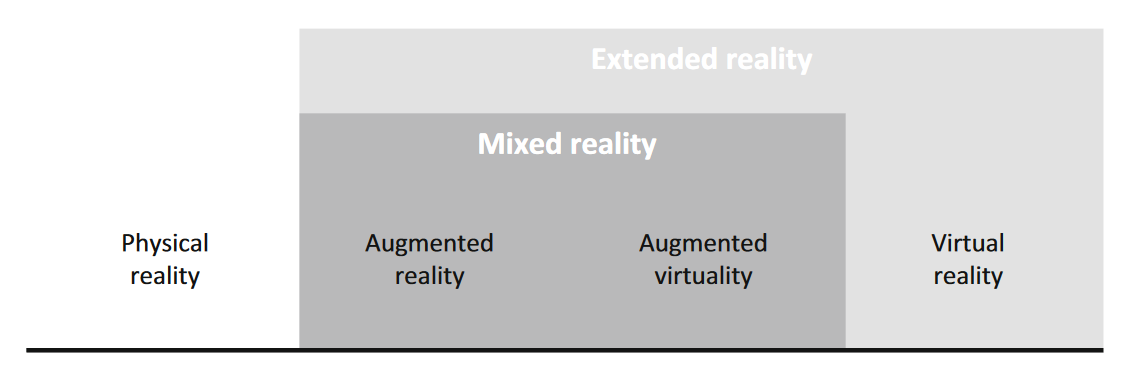
\includegraphics[width=0.95\textwidth]{images/Mixed-Reality-Cont-NEW.png}
 \caption{Reality-virtuality continuum nach \cite{wohlgenannt_virtual_2020}}
 \label{fig:continuum}
\end{figure}

Auf dem RVC bilden die reale Umgebung und die virtuelle
Umgebung die beiden Pole des Kontinuums. Die physikalische Realität setzt sich ausschließlich aus Elementen zusammen, welche durch eine Person direkt wahrgenommen werden können. Die virtuelle Umgebung, also die VR, besteht ausschließlich aus virtuellen Elementen. Der Nutzende wird dabei von der physikalischen Umgebung abgeschirmt, sodass er vollständig in die virtuelle Umgebung eintauchen kann. Der Bereich, der sich zwischen den beiden Polen des Kontinuums befindet, kombiniert virtuelle und physikalische Elemente und wird als Mixed Reality bezeichnet. Eine Umgebung, in der die physikalischen Elemente überwiegen, wird als Augmented Reality bezeichnet. Hierbei findet eine Erweiterung der physikalischen Realität durch virtuelle Elemente statt. Eine Erweiterung einer virtuellen Umgebung um physikalische Elemente wird demgegenüber als Augmented Virtuality bezeichnet. 
Ein weiterer Begriff, der in diesem Kontext häufig Verwendung findet, ist der Begriff der Extended Reality. Dieser wird häufig als Überbegriff verwendet und erfasst alle realen und virtuellen kombinierten Umgebungen und Mensch-Maschine-Interaktionen, die durch Computertechnologie und tragbare Geräte erzeugt werden (Fast-Berglund et al. 2018, S. 32). \citet{wohlgenannt_virtual_2020} haben daher das ursprüngliche RVC um diesen Begriff erweitert (vgl. \autoref{fig:continuum}). 
 
\subsection{Hardware - HMD und Controller}

\subsection{Motion Sickness}

Das Erleben von VR kann bei Nutzenden Symptome auslösen, die denen von Motion Sickness aus anderen Bereichen ähneln \citep{somrak_estimating_2019}. In der wissenschaftlichen Literatur werden neben dem Begriff "Motion Sickness" verschiedene Begriffe zur Beschreibung von unerwünschten Begleiterscheinungen virtueller Umgebungen verwendet. Dazu gehört der Begriff "Simulator Sickness", der insbesondere in den frühen militärischen Flugsimulatoren geprägt wurde (Kennedy et al., 1993), sowie "Cybersickness", das ursprünglich die Begleiterscheinungen virtueller Umgebungen allgemein beschrieb (McCauley und Sharkey, 1992). In Studien mit HMDs findet zudem der Begriff "VR-Sickness" Verwendung (Cobb et al., 1999; Kim et al., 2018). In der Forschung zu virtuellen Umgebungen werden diese Begriffe oft synonym verwendet, wobei eine spezifische Abgrenzung nicht erfolgt \citep{saredakis_factors_2020}. Im weiteren Verlauf dieser Arbeit wird der Begriff "Motion Sickness" verwendet. 

Das Spektrum der Symptome von Motion Sickness ist vielfältig. Zu den am häufigsten auftretenden Symptomen zählen unter anderem Unwohlsein, Apathie, Übelkeit, Schläfrigkeit, Desorientierung, Augenbelastung und Müdigkeit \citep{somrak_estimating_2019}. In besonders schweren Fällen können darüber hinaus Symptome wie Erbrechen, Schweißausbrüche, übermäßiger Speichelfluss, Schwindel, Magenschmerzen und völlige Arbeitsunfähigkeit auftreten \citep{kennedy_research_2010}. 

Die genauen Ursachen von Motion Sickness sind bislang nicht vollständig aufgeklärt. Eine der prominentesten Erklärungen liefert die Sensorische Konflikttheorie \citep{oman_motion_1990}. Diese besagt, dass die Symptome durch eine Diskrepanz zwischen visuellen, vestibulären und propriozeptiven Signalen entstehen. Diese Signale dienen in der Regel der Wahrnehmung der Ausrichtung und Bewegung des Körpers. In einer virtuellen Umgebung tritt jedoch häufig der Fall ein, dass der Körper visuell Bewegung wahrnimmt, während die vestibulären und propriozeptiven Systeme keine entsprechende Bewegung registrieren. Diese widersprüchlichen Signale führen zu sensorischen Diskrepanzen und können Motion Sickness auslösen. 

Als weitere Erklärungsansätze werden die Vergiftungstheorie sowie die Posturale Instabilitätstheorie diskutiert. Die Vergiftungstheorie besagt, dass der menschliche Körper bei der Aufnahme von Gift eine Reaktion auslöst, die das visuelle und vestibuläre System beeinflusst. In virtuellen Umgebungen können Reize das visuelle und vestibuläre System irritieren, sodass der Körper fälschlicherweise glaubt, Gift aufgenommen zu haben. Als Konsequenz treten unangenehme Symptome und eine Übelkeitsreaktion auf \citep{laviola_discussion_2000}. Die Posturale Instabilitätstheorie nach \citet{riccio_ecological_1991} basiert auf der Annahme, dass die Aufrechterhaltung der posturalen Stabilität in der Umgebung eines der Hauptziele menschlichen Verhaltens darstellt. Posturale Stabilität beschreibt den Zustand, in dem unkontrollierte Bewegungen der Wahrnehmungs- und Handlungssysteme minimiert werden. In virtuellen Umgebungen können abrupte oder signifikante Veränderungen zu einem Verlust der posturalen Kontrolle führen, insbesondere wenn die entsprechenden Kontrollstrategien noch nicht erlernt sind. Die Theorie besagt, dass anhaltende posturale Instabilität die Hauptursache für Motion Sickness ist. Je länger diese Instabilität andauert, desto schwerer sind die auftretenden Symptome.

Die Erfassung der Symptome von Motion Sickness erfolgt mittels subjektiver oder auch seltener objektiver Messmethoden \citep{somrak_estimating_2019}. Eine der am häufigsten verwendeten subjektiven Messmethoden ist der von \citet{kennedy_simulator_1993} entwickelte Simulator Sickness Questionnaire (SSQ) . Zu den objektiven Verfahren zählt die Messung physiologischer Veränderungen im menschlichen Körper, beispielsweise von Herzfrequenz, Blinkrate, Hauttemperatur oder Hirnstromaktivität (EEG), um Motion Sickness quantitativ zu erfassen \citep{somrak_estimating_2019}. 

\section{Barrierefreiheit (in VR)} 

Die Forschung zur Barrierefreiheit in VR ist ein noch junges Forschungsgebiet, das besonders in den letzten Jahren zunehmend an Aufmerksamkeit gewonnen hat. Häufig konzentrieren sich die Studien auf eine bestimmte Form der Barriere oder Einschränkung, wie Seh-, Hör-, motorische oder kognitive Beeinträchtigungen. Dabei werden die spezifischen Probleme und Herausforderungen identifiziert sowie entsprechende Konzepte und Lösungsansätze erarbeitet. Da sich diese Arbeit auf Menschen mit motorischen Einschränkungen bezieht, wird im Folgenden ein kurzer Überblick über den aktuellen Forschungsstand in diesem Bereich gegeben. 

\begin{itemize}
    \item Definition
    
    „Motor impairment is a loss or limitation of function in muscle control or movement or a limitation in mobility. Common causes include arthritis, paralysis, cerebral palsy, or repetitive strain injury. Motor impairment may also include difficulties in speech control and the need to use input devices other than a mouse or keyboard.“ ([Yuan et al., 2011, p. 83])
    
    \item Richtlinien/Guidelines: 
    
    „So far, guidelines for games rarely consider VR accessibility and few guidelines are exclusively made for VR applications. Many of them are specialized in one specific impairment or device. The way users interact with VR is hardly comparable with other software, so generalized guidelines can not be applied (Cairns et al., 2019a).“ ([Heilemann et al., 2021, p. 3])
    
    \begin{itemize}
        \item An October 2020 report from XRA (XR Association 2020) provides explicit guidance on the development of VR and AR applications that are accessible to disabled users.
        \item Oculus/Meta has also introduced Virtual Reality Check (VRC) guidelines related to accessibility - sind aber sehr beschränkt (z.B. playable without audio, should provide an option to be played with one hand and/or controller, display settings such as brightness and contrast, color blindness options, option to rotate their view without physically moving their head/neck, multiple locomotion styles when possible, provide a setting to enable users to perform all interactions and access information from a fixed position)  
        \item XR Access is a recently established community of university and industry partners focused on addressing the accessibility challenges encountered with VR and AR technologies (Ziel: Inclusive design and accessibility become an unremarkable part of all XR creation) 
        \item Accessibility Guidelines for VR Games - A Comparison and Synthesis of a Comprehensive Set (Heilemann et al.) - --> Zusammenfassung von bestehenden Guidelines mit Fokus auf Games im Allgemeinen, mit einem Absatz speziell für VR Games
    \end{itemize}
\end{itemize}

\subsection{Probleme}

TO DO - Kapiteleinleitung!

{\normalfont \bfseries 1. VR-Gerät einrichten, auf-/absetzten und tragen}  

Ein grundlegendes Problem für Menschen mit motorischen Einschränkungen bei der Nutzung von VR-Anwendungen stellt bereits die Einrichtung des Geräts dar, da dieser Prozess oft einen hohen körperlichen Einsatz oder auch feine motorische Fähigkeiten erfordert \citep{gerling_critical_2021}. So kann bereits das Einlegen der Batterien in die VR-Controller, das Anschließen von Kabeln an den Computer oder das Festlegen der Spielzeitbegrenzung eine Barriere darstellen \citep{mott_i_2020}. Auch das eigenständige Auf- und Absetzen eines VR-HMD sowie das Einstellen des Kopfbandes kann für Personen mit eingeschränkter Beweglichkeit der Arme oder des Oberkörpers eine erhebliche Herausforderung darstellen \citep{mott_i_2020}. 
Eine zusätzliche Barriere stellen HMDs mit Kabelverbindung zum Computer dar. Dies gilt sowohl für die Einrichtung des Gerätes als auch für die Nutzung. So kann es z.B. vorkommen, dass Personen die einen Rollstuhl benutzen, versehentlich über die Kabel fahren oder sich diese in den Reifen verfangen \citep{mott_i_2020, wong_survey_2017}. 

{\normalfont \bfseries 2. Annahmen bzgl. des Körpers} 
 
Die umfangreichen Anforderungen an die körperliche Beteiligung, die VR-Technologie stellt, können Barrieren für Menschen schaffen, die ihren Körper auf andere Weise in das System einbringen \citep{gerling_critical_2021}. Die geforderten Körperbewegungen basieren oft auf Fähigkeiten und Funktionen nicht-behinderter Personen. Dazu gehören beispielsweise die Nutzung im Stehen sowie die Verwendung von Gesten und beiden Hände zur Interaktion mit virtuellen Objekten \citep{wong_survey_2017}. VR-Anwendungen haben oft Probleme, Körper zu verfolgen und zu erfassen, die vom „Standard“ abweichen \citep{wong_survey_2017}. Darüber hinaus basieren auch anwendungsintere Anforderungen an Energie und Ausdauer auf den Fähigkeiten nicht-behinderter Menschen, was Personen mit Erschöpfung oder chronischen Schmerzen von der Verwendung ausschließt \citep{wong_survey_2017}. 

{\normalfont \bfseries 3. Controller } 

Die Nutzung gängiger VR-Controller stellt für Personen mit motorischen Einschränkungen eine erhebliche Herausforderung dar. Aktuelle VR-Systeme sind in erster Linie für Kernnutzende konzipiert, die zwei Hände verwenden, lange stehen und virtuelle Objekte mit Hilfe der Hände manipulieren können. Diese Anforderungen schließen viele Menschen mit motorischen Einschränkungen grundsätzlich von der Nutzung aus \citep{dombrowski_designing_2019}. Zusätzlich wird in VR-Anwendungen oftmals der gesamte Bewegungsradius der Nutzenden ausgenutzt und es werden Eingaben über Kopfhöhe sowie Bewegungen und Drehungen des Oberkörpers gefordert \citep{gerling_critical_2021}. Insbesondere die Nutzung von VR-Controller setzt dabei voraus, dass Nutzende eine oder beide Hände mit vollständiger Finger-, Handgelenks- und Armbeweglichkeit zur Verfügung haben \citep{mott_accessible_2019}. Daher haben viele Nutzende mit motorischen Einschränkungen Schwierigkeiten, die Tasten auf den Motion-Controllern zu erreichen, zu drücken und gedrückt zu halten, insbesondere wenn gleichzeitig mehrere Tasten betätigt werden müssen \citep{mott_i_2020}. Zusätzlich müssen die Controller stets im Sichtfeld der Headset-Kameras bleiben, damit ihre Position korrekt erfasst werden kann, was eine weitere Herausforderung darstellt \citep{mott_i_2020}. Für Personen, die nur wenig bis gar keine Beweglichkeit der Arme oder Hände haben, sind VR-Controller komplett unzugänglich \citep{mott_i_2020}.



\subsection{Lösungsansätze}
In der Literatur werden bereits einige Ansätze zur Verringerung der genannten Barrieren vorgestellt. So argumentieren \citet{mott_i_2020} bzgl. der Herausforderungen hinsichtlich der gängigen HMDs, dass Drehknöpfe zum Anpassen des Kopfbandes näher an der Vorder- oder Seite des Headsets positioniert werden sollten, um die Erreichbarkeit zu verbessern. Eine automatische Anpassung des Kopfbandes anstelle einer manuellen Einstellung wäre ebenfalls hilfreich. Des Weiteren könnte die Verwendung eines kabellosen HMD eine einfache Lösung darstellen, um die Bewegungsfreiheit der Nutzenden zu erhöhen. Hinsichtlich der Interaktionsmöglichkeiten wird die Bereitstellung einer größeren Auswahl an Optionen und Anpassungsmöglichkeiten für Controller vorgeschlagen, um den unterschiedlichen Bedürfnissen der Nutzenden gerecht zu werden. Darüber hinaus könnten Eingabemethoden wie Sprachsteuerung und Blicksteuerung eine zugängliche Alternative zu den herkömmlichen Motion-Controllern darstellen. Des Weiteren wird vorgeschlagen, dass Nutzende die Möglichkeit haben sollten, Interaktionsstile oder Steuerungen neu zu konfigurieren, um eine individuellere Nutzung zu ermöglichen. \citet{dombrowski_designing_2019} führen weiter aus, dass weitere potenzielle Verbesserungen die Steuerung von VR-Anwendungen mit alternativen Eingabegeräten wie Schaltern und die Verwendung von Einstellknöpfen an VR-HMDs, die sich automatisch anpassen können, umfassen könnten. Des Weiteren sollten Anwendungen und Eingabegeräte in der Lage sein, ungleichmäßige Eingaben zu tolerieren und sich bemühen, die Absicht des Nutzenden zu interpretieren. Das Design der Anwendung und die Interaktionsformen sollten effizient und komfortabel sein und mit minimaler Ermüdung verwendet werden können. 
Neben diesen theoretischen Lösungsansätzen wurden in der Forschung bisher nur wenige praktische Untersuchungen für alternative Eingabemethoden durchgeführt. Bei diesen Untersuchungen liegt der Fokus oftmals auf Sprach- und Blicksteuerung. Beispielsweise untersuchten und vergleichen \citet{minakata_pointing_2019} alternative Eingabeoptionen wie Kopf-, Blick- und Fußsteuerung hinsichtlich mentaler und physischer Anstrengung sowie Präzision. \citet{wang_intelligent_2018} hingegen entwickelten und evaluierten ein Eingabesystem, das auf Gesichtsausdrücken und Augenbewegungen basiert. \citet{10.1145/3441852.3471230} entwickelten Nearmi, ein Interaktionssystem, das darauf abzielt, die Bewegungen des Oberkörpers und des Kopfes zu reduzieren und das Auffinden und Erreichen von Points of Interest in der virtuellen Umgebung zu erleichtern. Dieses Framework basiert jedoch weiterhin überwiegend auf Eingaben mittels VR-Controller. Die Integration von Schaltern jeglicher Form zu Interaktion mit VR-Anwendungen wird in der Literatur bisher kaum betrachtet.

\section{Binäre Interaktionsschnittstellen}

TO DO: Kapiteleinleitung 

\subsection{Switches}

„Binary input is the smallest amount of interaction that can be provided with a switch, because holding down the switch for a certain amount of time may be impossible for a sip and puff device or painful for someone with arthritis.“ ([Yuan et al., 2011, p. 88])

„A switch is an assistive technology device that replaces the use of a mouse, keyboard, controller or joystick which severely motor impaired players may find difficult to use. Switches can be operated by any body part that is able to produce consistent and voluntary movement, and different types of switches can be identified based upon the type of action required to use them (sip and puff, pull, push, or squeeze). Individuals with severe motor impairments may sometimes be able to use only one switch, whereas individuals with less severe motor impairments may be able to use multiple switches.“ ([Yuan et al., 2011, p. 88])

\begin{itemize}
    \item Schalter/Knöpfe 
    \item Sip and Puff 
    \item Klicken/Geräusche 
    \item noch was? 
\end{itemize}

\subsection{Scanning-Verfahren}
Scanning ist eine Eingabemethode, bei der dem Nutzenden eine Auswahl an Selektionsoptionen auf einem Display präsentiert wird. Sobald das gewünschte Element angezeigt wird, erfolgt eine Interaktion durch den Nutzenden, um dieses auszuwählen. Typischerweise wird dafür ein einzelner Schalter oder ein Array aus zwei oder mehr Schaltern verwendet. Scanning ermöglicht eine interaktive Steuerung, ohne dass umfangreiche motorische Fähigkeiten erforderlich sind.

Es existieren diverse Scanning-Verfahren, die sich in der Art und Weise der Durchlaufung der Auswahlmöglichkeiten voneinander unterscheiden. Die gängigsten Verfahren sind dabei das Item Scanning, welches sich in den Unterarten Automatic, Step und Inverse Scanning differenziert, sowie das Continuous Cartesian Scanning.

Beim Item Scanning erfolgt eine sukzessive Hervorhebung einzelner Elemente. Die Selektion eines gewünschten Elements erfolgt durch Betätigung eines Schalters, sofern das entsprechende Zielelement hervorgehoben ist. 

{\normalfont \bfseries Automatic Item Scanning} 

Beim Automatic Item Scanning erfolgt die Hervorhebung der Elemente automatisch. Die Hervorhebung bleibt bei jedem Element für ein vordefiniertes Zeitintervall stehen. Wird während der Hervorhebung eines Elementes eine Benutzereingabe vorgenommen, wird das hervorgehobene Element ausgewählt. Andernfalls wandert die Hervorhebung zum nächsten Element.
Der wesentliche Vorteil des Automatic Item Scannings besteht in der Möglichkeit, die Interaktionen des Nutzenden auf ein Minimum zu reduzieren. Allerdings ist das Verfahren insgesamt relativ langsam. Des Weiteren erfordert es ein hohes Maß an sensorischer und kognitiver Aufmerksamkeit, um die Reihenfolge der Hervorhebung zu beobachten und zu verfolgen.

{\normalfont \bfseries Step Item Scanning} 

Beim Step Item Scanning erfolgt die Hervorhebung der Elemente nicht automatisch, sondern durch wiederholte Aktivierung des Schalters durch den Nutzenden. Mit jeder Aktivierung erfolgt ein Sprung zur nächsten Auswahlmöglichkeit, bis das gewünschte Element erreicht ist. Die Selektion kann entweder mittels eines zusätzlichen Schalters getroffen werden, oder das System akzeptiert die Auswahl nach Ablauf einer festgelegten Zeitspanne (Dwell Selection). Ein wesentlicher Vorteil des Step Item Scannings besteht in der Möglichkeit, dass die Nutzenden die Geschwindigkeit der Hervorhebung selbst steuern können. Dadurch ist das Verfahren insgesamt schneller als das Automatic Item Scanning.  Allerdings ist zu berücksichtigen, dass dieses Vorgehen eine wiederholte Aktivierung des Schalters erfordert, was mit einer motorischen Ermüdung einhergehen kann.

{\normalfont \bfseries Inverse Item Scanning} 

Die Initiierung des Inverse Scanning erfolgt durch Aktivierung und kontinuierliches Halten des Schalters. Solange die Betätigung des Schalters aufrechterhalten wird, erfolgt der Scan der Elemente. Sobald das gewünschte Element hervorgehoben wird, kann die Person den Schalter loslassen, um die Auswahl zu bestätigen. Inverse Scanning erfordert im Vergleich zum Step Scanning eine geringere Anzahl an Aktivierungen des Schalters, ist jedoch mit einer höheren sensorischen und kognitiven Aufmerksamkeit verbunden, da das Scanning kontinuierlich überwacht werden muss. Insbesondere für Personen, die einen erhöhten Zeitaufwand für die Initiierung und Ausführung von Bewegungen benötigen, kann dieses Verfahren von Vorteil sein. 

{\normalfont \bfseries Continuous Cartesian Scanning}

Im Rahmen des Continuous Cartesian Scannings erfolgt das Scannen entlang orthogonaler Richtungen, bis das jeweilige Ziel erreicht ist. Eine horizontale Scanlinie beginnt mit einem kontinuierlichen Scan vom oberen Rand des Sichtfelds nach unten.  
Sobald die Scanlinie das Zielobjekt kreuzt, aktiviert der Nutzende den Schalter, wodurch die horizontale Linie an ihrer Position sichtbar bleibt. In der Folge wird eine vertikale Scanlinie initiiert, welche kontinuierlich von der linken Seite des Sichtfelds nach rechts scannt. Wenn auch die vertikale Scanlinie das Zielobjekt kreuzt, aktiviert der Nutzende den Schalter, um dieses Objekt auszuwählen.

Der wesentliche Vorteil des Scannings liegt darin, dass eine Selektion von Elementen mit minimalem motorischen Aufwand realisierbar ist. Allerdings setzt die Nutzung dieser Methode gute visuelle Fähigkeiten, hohe Aufmerksamkeit sowie die Fähigkeit voraus, die Abfolge der Auswahlmöglichkeiten zu erfassen, insbesondere im Kontext des Item Scannings. Des Weiteren ist Scanning im Vergleich zu anderen Eingabemethoden relativ langsam. Um diesen Nachteil zu kompensieren, wurden verschiedene Ansätze zur Beschleunigung des Scannings entwickelt. Eine zentrale Methode ist das sogenannte Rate Enhancement beim Item Scanning, bei dem Elemente zu Gruppen zusammengefasst und selektiert werden können. Dadurch kann der Auswahlprozess signifikant beschleunigt werden. 
Darüber hinaus stellt die Festlegung der optimalen Scangeschwindigkeit (Scan Rate) eine der größten Herausforderungen beim Scanning dar. Eine zu hohe Scan Rate kann dazu führen, dass Nutzende Schwierigkeiten haben, im richtigen Moment eine Auswahl zu treffen. Eine zu niedrige Scan Rate hingegen verzögert den Eingabeprozess unnötig. Als bewährte Richtlinie zur Optimierung der Scan Rate kann die sogenannte 0,65-Regel herangezogen werden. 

\section{Usability und User Experience}

\section{PaneoVR}

\section{Zusammenfassung} 

Jedes Kapitel sollte mit einer eigenen Zusammenfassung abschließen (vielleicht
ausgenommen dem einleitenden Kapitel). Der einleitende Text des Kapitels und die
Zusammenfassung bilden zugleich eine Klammer um das Kapitel und zeigen einen
roten Faden im Übergang zwischen den Kapiteln auf. 

Das wesentliche bei der Zusammenfassung insbesondere im Kapitel {\emph Stand der
Forschung} ist es, das im Kapitel beschriebene in eigenen Worten kurz und prägnant
darzustellen und in Bezug zur eigenen Arbeit zu setzen.

Es könnte in der Zusammenfassung zum Beispiel stehen: \glqq Wie X und Y gezeigt
haben, ist noch offen, wie... In dieser Arbeit soll diese Frage so und so
angegangen werden.\grqq Oder \glqq Wie gezeigt werden konnte, gibt es derzeit für X
noch keine (zufriedenstellende) Lösung...\grqq.
